
The evaluation of the proposed refinement and axiom weakening operator has been carried out using the implementation described in \cref{prototype} using different ontologies from BioPortal \cite{whetzel2011bioportal,bioportal}. Additionally, the pizza ontology \cite{pizzaontology} was included in the testing. The chosen ontologies are of different sizes and use a varying amount of expressive features. Some characteristics of the used ontologies are shown in \cref{table:ontologies}. On average, they contain about 289 axioms, 73 concept names, 29 role names, and 168 subconcepts. Some additional evaluation results, that did not fit into this chapter, can be found in \cref{eval-appendix}.

\begin{table}[ht]
  \scriptsize
  \centering
  \addtolength{\tabcolsep}{-0.75mm}
  \begin{tabular}{|l|llrrrr|}
    \hline
    Abbreviation & Name & Expressivity & Axioms & Concepts & Roles & Subcon. \\
    \hline
    admin & Nurse Administrator & $\mathcal{ALCHOIF}$ & 229 & 42 & 29 & 144 \\
    ahso & Animal Health Surveillance Ontology & $\mathcal{ALCRIF}$ & 166 & 38 & 31 & 104 \\
    cdao & Comparative Data Analysis Ontology & $\mathcal{ALCROIQ}$ & 437 & 132 & 68 & 375 \\
    cdpeo & Chronic Disease Patient Education & $\mathcal{ALCHF}$ & 422 & 41 & 31 & 170 \\
    covid19-ibo & Covid-19 Impact on Banking Ontology & $\mathcal{ALCH}$ & 288 & 160 & 33 & 227 \\
    ecp & Electronic Care Plan & $\mathcal{ALCRQ}$ & 127 & 33 & 17 & 99 \\
    emo & Enzyme Mechanism Ontology & $\mathcal{ALCHQ}$ & 368 & 157 & 24 & 255 \\
    evi & Evidence Graph Ontology & $\mathcal{ALCRI}$ & 143 & 30 & 38 & 69 \\
    falls & Falls Prevention & $\mathcal{ALCH}$ & 79 & 30 & 20 & 35 \\
    fo & Fern Ontology & $\mathcal{ALCHI}$ & 59 & 31 & 4 & 46 \\
    gbm & Glioblastoma & $\mathcal{ALCIF}$ & 603 & 108 & 28 & 227 \\
    gfvo & Genomic Feature and Variation Ontology & $\mathcal{ALCH}$ & 332 & 102 & 30 & 170 \\
    koro & Knowledge Object Reference Ontology & $\mathcal{ALCHI}$ & 262 & 110 & 19 & 194 \\
    lico & Liver Case Ontology & $\mathcal{ALCHQ}$ & 366 & 93 & 36 & 230 \\
    mamo & Mathematical Modelling Ontology & $\mathcal{ALCR}$ & 229 & 107 & 3 & 154 \\
    mpio & Minimum PDDI Information Ontology & $\mathcal{ALCH}$ & 38 & 30 & 14 & 45 \\
    pizza & Pizza Ontology & $\mathcal{SHOIN}$ & 1131 & 100 & 8 & 376 \\
    provo & Provenance Ontology & $\mathcal{ALCRIN}$ & 170 & 31 & 42 & 128 \\
    qudt & Quantities, Units, Dimensions, and Types & $\mathcal{SHOIQ}$ & 293 & 74 & 73 & 177 \\
    trans & Nurse Transitional & $\mathcal{ALCROIF}$ & 244 & 44 & 22 & 123 \\
    triage & Nurse triage & $\mathcal{ALCHF}$ & 132 & 33 & 29 & 129 \\
    vio & Vaccine Investigation Ontology & $\mathcal{ALCRI}$ & 249 & 81 & 44 & 235 \\
    \hline
  \end{tabular}
  \caption{The ontologies used for evaluation. The number of axioms, concept names, role names, and subconcepts are taken after applying preprocessing.}
  \label{table:ontologies}
\end{table}

Since the ontologies use OWL 2, the axioms and concepts do not map directly to \SROIQ. It is possible to directly apply axiom weakening to OWL 2 DL ontologies, a description of such a scheme and why it might be useful can be found in \cref{weakening-owl-2-dl}. However, in order to follow the definitions laid out in \cref{weakening-sroiq}, the OWL 2 DL axioms have been mapped to \SROIQ axioms. A detailed description of the mapping between OWL 2 DL and \SROIQ used for this evaluation can be found in \cref{owl-to-sroiq}. While some axioms have a direct mapping, others have been replaced by a set of axioms that together are equivalent. During the preprocessing, we further removed annotation axioms and axioms related to data properties and any axiom that caused any OWL 2 DL profile violation, as our weakening operator does not handle them.

Claims about runtime should generally only be used for relative comparisons and rough estimates. While they will obviously vary greatly based on hardware choices, all evaluations here have been performed on an Intel Coffee Lake system running at around 4GHz for the duration of the experiment. Unless otherwise indicated, the FaCT++ reasoner \cite{tsarkov2006fact++,factpp} was used for evaluation.

\section{Evaluating the Quality of Repairs}\label{eval-quality}


In order to evaluate the proposed approach of axiom weakening, specifically for its application in the context of automatic repair of ontologies, we need a way to compare the quality of different possible repairs. As has already been discussed in \cite{troquard2018repairing}, the problem of deciding which of two possible repaired ontologies $\Omc_1$ or $\Omc_2$ is preferable is not generally well-defined. As such, this thesis will use the same measure defined for the experimental evaluation in \cite{troquard2018repairing}. The main idea is to use the size of the \emph{inferred class hierarchy} to evaluate the amount of ``information'' a repair can retain.

\begin{definition}\label{def:inf}
  The \emph{inferred class hierarchy} of an ontology $\Omc$ is given by
  \begin{align*}
    \Inf(\Omc) = \{ A \sqsubseteq B \mid A, B \in N_C \text{ and } A \sqsubseteq_\Omc B \} \enspace.
  \end{align*}
\end{definition}

To compare the relative amount of ``information'' between two ontologies, we compare them based on their differences in the inferred class hierarchy. We use for this purpose the \emph{inferable information content} (IIC) as defined in \cite{troquard2018repairing}.

\begin{definition}\label{def:iic}
  The \emph{inferable information content} of an ontology $\Omc_1$ with respect to another ontology $\Omc_2$ is given by
  \begin{align*}
    \qual(\Omc_1, \Omc_2) = \frac{| \Inf(\Omc_1) \setminus \Inf(\Omc_2) |}{|\Inf(\Omc_1) \setminus \Inf(\Omc_2)| + |\Inf(\Omc_2) \setminus \Inf(\Omc_1)|} \enspace,
  \end{align*}
  where $|X|$ is the cardinality of the set $X$.
\end{definition}

The IIC of an ontology $\Omc_1$ with respect to a second ontology $\Omc_2$, written $\qual(\Omc_1, \Omc_2)$, is a number between $0$ and $1$. A value closer to $0$ indicates that $\Omc_1$ contains more ``information'' than $\Omc_2$, while a value towards $1$ indicates the opposite. Inferred hierarchy axioms common to both ontologies do not influence the results, and if $\Omc_2$ is entailed by $\Omc_1$, then the IIC of $\Omc_1$ with respect to $\Omc_2$ is always $1$. If both $\Omc_1$ and $\Omc_2$ have some inferences that are not shared by the other ontology, the IIC will be strictly between $0$ and $1$. Note that if the cardinality of the inferred class hierarchy is larger for one ontology, then it will also be the one preferred by the IIC. Some weaknesses of this measure when it comes to evaluating repairs, like the fact that only atomic concepts are considered, have already been discussed in \cite{troquard2018repairing}. For the case of repairing \SROIQ ontologies, this is even more relevant, since the role hierarchy is entirely ignored.

The evaluation starts by first making the ontologies inconsistent. This has been achieved by repeatedly adding axioms to the ontology until it was no longer consistent. The newly added axioms were generated by strengthening randomly selected axioms of the ontology. Axioms are strengthened by applying an axiom strengthening operator, that is equivalent to the axiom weakening operator in \cref{def:weaken}, except for swapping the generalization and specialization operators and not using $\bot \sqsubseteq \top$ to remove the axiom. An axiom $\alpha'$ is stronger than another axiom $\alpha$ with respect to the ontology $\Omc$ if $\alpha' \models_\Omc \alpha$. Note that this is only a useful characterization if $\alpha \not\in \Omc$. It was ensured that the added axioms on their own were not inconsistent. After making the ontology inconsistent, it was repaired using different automatic repair algorithms. Each inconsistent ontology was repaired once with the repair algorithm using the axiom weakening operator presented in \cref{algo:repair-weaken} and once using \cref{algo:repair-remove}. As can be seen in \cref{ex:alc-weakening}, choosing a maximal consistent subset can sometimes lead to less information loss than using the weakening based algorithm. To experimentally evaluate how good weakening performs against the maximal consistent subset based repair on average, the repair was also performed by selecting a randomly sampled maximal consistent subset.

\begin{algorithm}[ht]
  \begin{algorithmic}
    \While{$\Omc$ is inconsistent}
      \State $\phi_\textnormal{bad} \gets \textsc{FindBadAxiom}(\Omc)$
      \State $\Omc \gets \Omc \setminus \{\phi_\textnormal{bad}\}$
    \EndWhile
    \State Return $\Omc$
  \end{algorithmic}
  \caption{\textsc{RepairOntologyRemove}($\Omc$)}
  \label{algo:repair-remove}
\end{algorithm}

This process, both making the ontology inconsistent and repairing it, was repeated one hundred times for each ontology, and the IIC was computed between the results of the different repair methods. The evaluation was performed using a randomly sampled maximal consistent subset as the reference ontology and by randomly sampling $16$ minimal inconsistent subsets during the selection of bad axioms in \textsc{FindBadAxiom}(\Omc). To obtain comparable results, both \textsc{RepairOntologyRemove}($\Omc$) and \textsc{RepairOntologyWeakening}($\Omc$) use the same implementation of \textsc{FindBadAxiom}($\Omc$). While the utilized OWL 2 DL reasoners are all highly optimized, they exhibit undesirable performance in some edge cases. Mostly they are fast to perform reasoning tasks like checking for consistency or entailment in the selected ontologies. However, when performance pitfalls are encountered, they may require significantly more time, making the computation required for repair unreasonably slow. For this reason, a timeout of 5 minutes was placed on the repairs execution and the outputs of runs that did not complete within this time limit were discarded and replaced by new runs. The results of these experiments are listed in \cref{table:results} and shown in \cref{fig:results-remove} and \cref{fig:results-mcs}.

\begin{table}[ht]
  \scriptsize
  \centering
  \begin{tabular}{|l|cc@{ }c|}
    \cline{2-4}
    \multicolumn{1}{l|}{} & IIC w.r.t. removal & \multicolumn{2}{c|}{IIC w.r.t. maximal consistent subset} \\
    \hline
    admin & 0.56 [0.51, 0.60] & 0.39 [0.33, 0.45] & (0.51 [0.45, 0.57]) \\
    ahso & 0.57 [0.52, 0.62] & 0.52 [0.47, 0.56] & (0.64 [0.59, 0.69]) \\
    cdao & 0.54 [0.49, 0.61] & 0.51 [0.44, 0.57] & (0.55 [0.48, 0.61]) \\
    cdpeo & 0.50 [0.47, 0.53] & 0.25 [0.20, 0.30] & (0.39 [0.33, 0.45]) \\
    covid19-ibo & 0.71 [0.67, 0.75] & 0.62 [0.58, 0.66] & (0.72 [0.68, 0.76]) \\
    ecp & 0.75 [0.70, 0.80] & 0.36 [0.30, 0.42] & (0.50 [0.44, 0.56]) \\
    emo & 0.68 [0.63, 0.72] & 0.61 [0.56, 0.65] & (0.73 [0.68, 0.77]) \\
    evi & 0.51 [0.46, 0.55] & 0.58 [0.53, 0.63] & (0.71 [0.66, 0.75]) \\
    falls & 0.75 [0.70, 0.81] & 0.50 [0.44, 0.57] & (0.60 [0.54, 0.66]) \\
    fo & 0.53 [0.48, 0.58] & 0.68 [0.63, 0.73] & (0.67 [0.62, 0.73]) \\
    gbm & 0.59 [0.54, 0.64] & 0.54 [0.49, 0.59] & (0.68 [0.63, 0.73]) \\
    gfvo & 0.53 [0.47, 0.58] & 0.54 [0.49, 0.59] & (0.71 [0.67, 0.75]) \\
    koro & 0.53 [0.48, 0.58] & 0.38 [0.32, 0.43] & (0.53 [0.47, 0.59]) \\
    lico & 0.53 [0.48, 0.59] & 0.51 [0.46, 0.57] & (0.63 [0.58, 0.68]) \\
    mamo & 0.55 [0.49, 0.61] & 0.64 [0.58, 0.69] & (0.72 [0.66, 0.77]) \\
    mpio & 0.69 [0.65, 0.74] & 0.70 [0.66, 0.75] & (0.70 [0.65, 0.74]) \\
    pizza & 0.56 [0.51, 0.62] & 0.57 [0.51, 0.63] & (0.63 [0.58, 0.69]) \\
    provo & 0.51 [0.47, 0.56] & 0.55 [0.51, 0.60] & (0.64 [0.60, 0.69]) \\
    qudt & 0.96 [0.93, 0.98] & 0.47 [0.40, 0.53] & (0.56 [0.49, 0.62]) \\
    trans & 0.56 [0.51, 0.61] & 0.41 [0.35, 0.47] & (0.51 [0.45, 0.57]) \\
    triage & 0.51 [0.46, 0.56] & 0.52 [0.47, 0.57] & (0.63 [0.57, 0.68]) \\
    vio & 0.48 [0.41, 0.54] & 0.50 [0.44, 0.57] & (0.57 [0.51, 0.63]) \\
    \hline
    Overall & 0.60 [0.58, 0.61] & 0.52 [0.50, 0.53] & (0.61 [0.60, 0.63]) \\
    \hline
  \end{tabular}
  \caption{Results of the evaluation. IIC is given as mean and 95\% confidence interval in brackets. The values in parentheses are for weakening that does not weaken the axioms in the maximal consistent subset chosen as reference ontology.}
  \label{table:results}
\end{table}

\begin{figure}[ht]
  \centering
  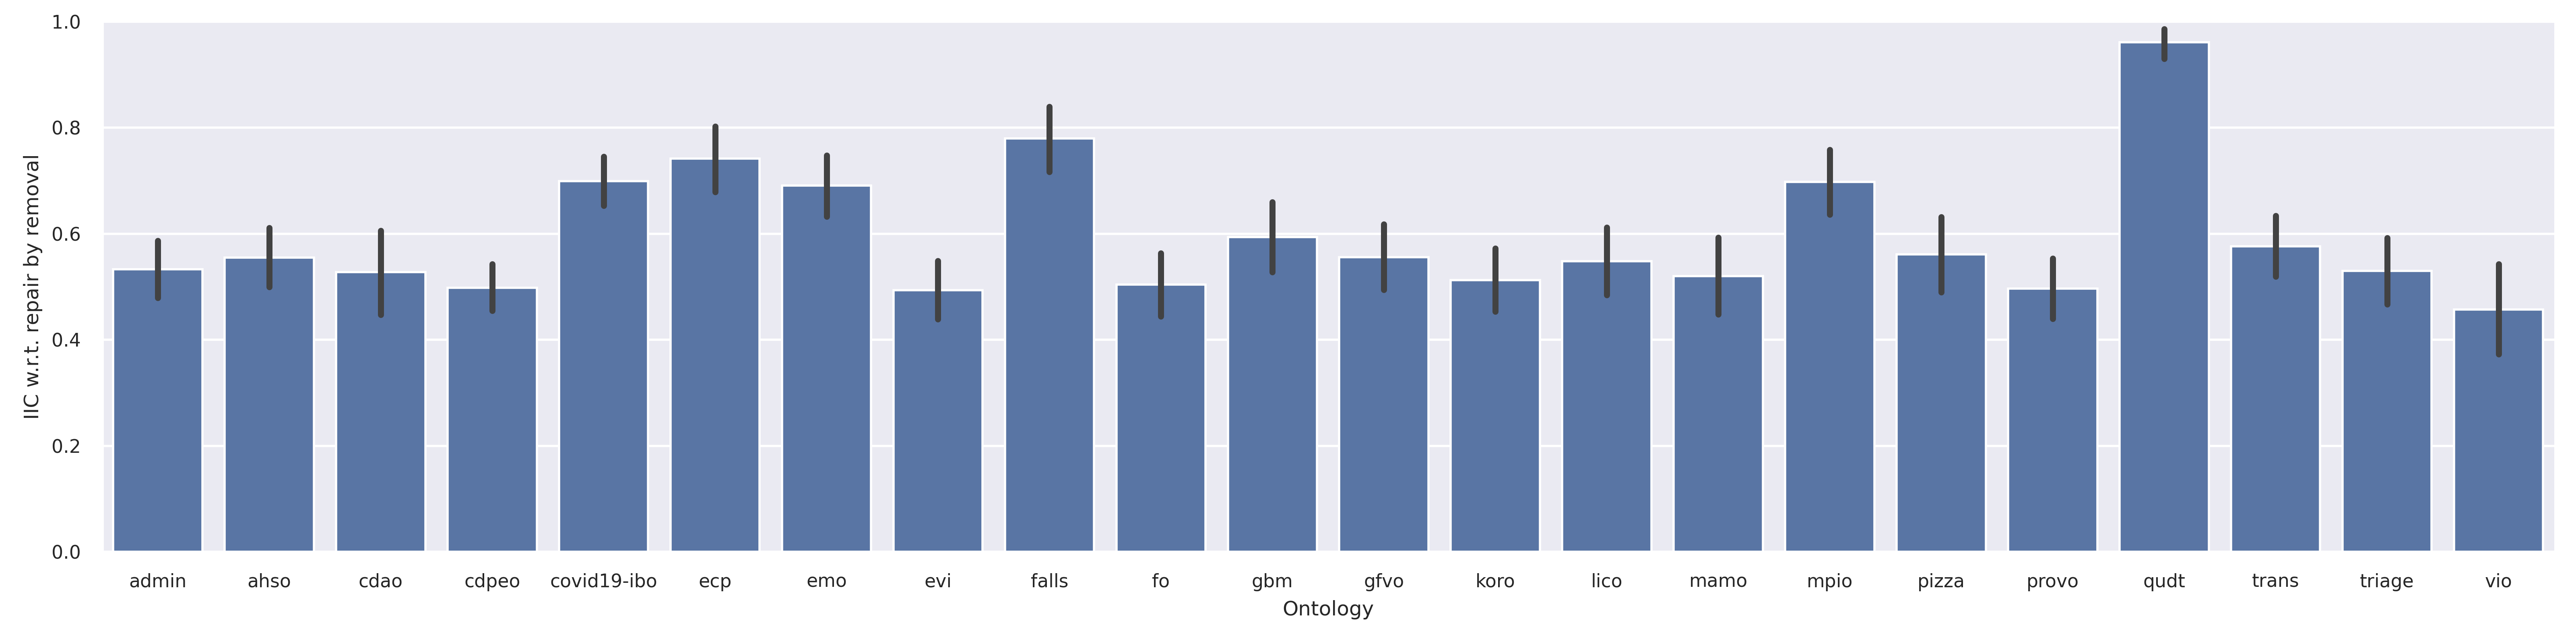
\includegraphics[width=\textwidth]{resources/iic-remove-ontology-bar.png}
  \caption{Mean IIC with respect to repair via removal per ontology. The error bars show the 95\% confidence interval.}
  \label{fig:results-remove}
\end{figure}

The results of the evaluation suggest that the repair by weakening is on average about as good or better than the repair by removal of axioms. While this supports the conclusion in \cite{troquard2018repairing} that weakening is able to retain more information than removal, the observed advantage was worse than what has been observed in \cite{troquard2018repairing}.

\begin{figure}[ht]
  \centering
  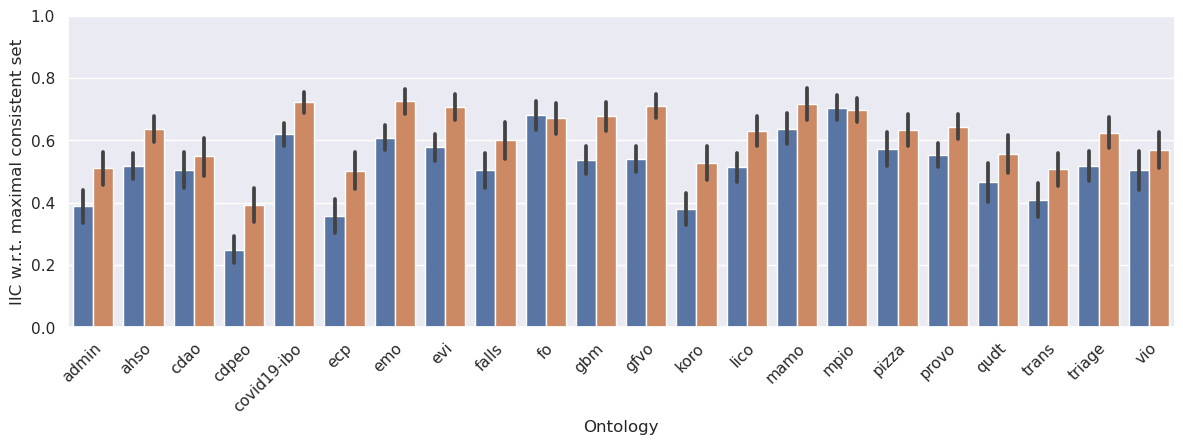
\includegraphics[width=\textwidth]{resources/iic-both-mcs-ontology-bar.png}
  \caption{Mean IIC with respect to a random maximal consistent subset. The error bars show the 95\% confidence interval. The orange bars used a variation of the repair by weakening, where axioms in the reference ontology are never weakened.}
  \label{fig:results-mcs}
\end{figure}

In contrast, it can be seen that the repair using weakening is not, in general, better than choosing a random maximal consistent subset. There are ontologies for which the repair by weakening is on average significantly worse when comparing using IIC. This is, however, a somewhat unequal comparison. We have seen in \cref{ex:alc-weakening} also a situation in which weakening performs worse when it comes to preserving information compared to choosing a maximally consistent subset. A more equal comparison, yet still not perfect since the maximal consistent subset for the reference ontology is not chosen uniformly at random, would be to a repair algorithm that starts with the reference ontology and uses weakening to add more information from the remaining axioms. This has been implemented and evaluated, and the results can be seen as the orange bars in \cref{fig:results-mcs}. Still, this result suggests that the heuristic used for selecting bad axioms is not reliable for preserving information, at least when measured using IIC. It has not been closely studied what causes the repair by weakening to significantly lose for some ontologies while being clearly preferred in others. Interestingly, there are also some cases in which the weakening based repair performs better against a random maximal consistent subset than against the repair by removal.

To overcome some weaknesses of the IIC, especially that it does not account for subsumptions between roles or complex concept expressions, tests were also carried out using an extended version of the inferred class hierarchy and IIC, adding to it subsumptions between subconcepts and roles.

\begin{definition}
  The \emph{extended inferred class hierarchy} of an ontology $\Omc$ is given by
  \begin{align*}
    \Inf^+(\Omc) ={} & \{ C \sqsubseteq D \mid C, D \in \sub(\Omc) \text{ and } C \sqsubseteq_\Omc D \} \\
    & \cup \{ R \sqsubseteq S \mid R, S \in \Lmc(N_R) \text{ and } R \sqsubseteq_\Omc S \} \enspace.
  \end{align*}
  The \emph{extended inferable information content} (IIC$^+$) of an ontology $\Omc_1$ with respect to another ontology $\Omc_2$ is given by
  \begin{align*}
    \qual^+(\Omc_1, \Omc_2) = \frac{| \Inf^+(\Omc_1) \setminus \Inf^+(\Omc_2) |}{|\Inf^+(\Omc_1) \setminus \Inf^+(\Omc_2)| + |\Inf^+(\Omc_2) \setminus \Inf^+(\Omc_1)|} \enspace,
  \end{align*}
\end{definition}

Of course, this new measure still only captures a small part of all consequences, but it should provide more accurate results when it comes to information about subconcepts and roles. When evaluating the experiment outcomes, we see that the values produced by IIC and IIC$^+$ are very similar. As may be expected, the repair by weakening is preferred slightly more strongly when using IIC$^+$. \Cref{fig:results-eiic} shows the comparison between IIC and IIC$^+$ for repair using axiom weakening w.r.t. repair by removal. The differences between IIC and IIC$^+$ are somewhat stronger when comparing against the repair using a random maximal consistent subset, but the differences are still not particularly noteworthy.

\begin{figure}[ht]
  \centering
  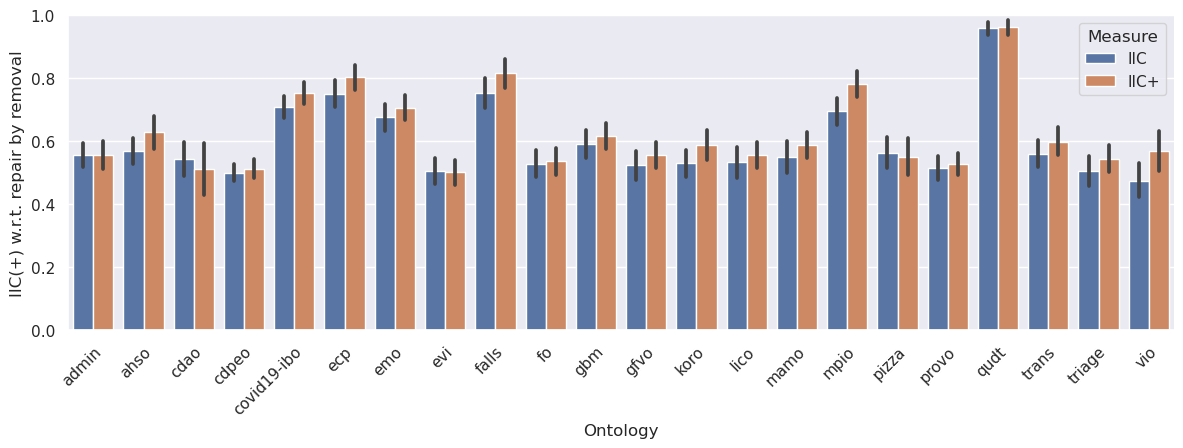
\includegraphics[width=\textwidth]{resources/iic-eiic-ontology-bar.png}
  \caption{Mean IIC and IIC$^+$ with respect to repair by removal per ontology. The error bars show the 95\% confidence interval.}
  \label{fig:results-eiic}
\end{figure}


\section{Effectiveness of Caching in Cover Computation}


As discussed in \cref{cache-impl}, to accelerate the computation of upward and downward covers, a cache was added to avoid repeated calls to the reasoner when the necessary information can already be inferred from previous computations. This section will discuss the experiments performed to evaluate the effectiveness of this cache.

Three versions of the upward and downward cover have been considered, the uncached version that calls the reasoner for every subsumption query, a version that caches only the exact queries that were already made previously, and finally the version that additionally infers some additional information from the transitivity of subsumption as listed in \cref{algo:cached-subs}. The experiment uses some of the same ontologies as have been used for the previously discussed evaluation of the repair quality. From the logical axioms of each ontology were selected, uniformly at random, one hundred groups with a fixed number of axioms. The same axioms may be selected multiple times. Each of the groups was then tested with a separate instance of the cache. The rationale behind testing with different group sizes is that the cache will obviously have a greater impact when the same cache can be reused for more cover computations. In each test run, the axiom weakening operator was applied to each axiom and the number of reasoner calls and (real) time taken were measured. The weakening operator used the complete (after preprocessing) ontology as the reference ontology. The test has further been performed using different OWL 2 DL reasoners. The final results of the evaluation can be seen in \cref{table:results-cache-calls} and are visualized in \cref{fig:results-cache-calls} and \cref{fig:results-cache-time}. Note that a logarithmic y-axis has been used for both plots.

\begin{table}[ht]
  \scriptsize
  \centering
  \begin{tabular}{|l|rrr|rrr|rrr|}
    \cline{2-10}
    \multicolumn{1}{l|}{} & \multicolumn{9}{c|}{\hspace{-4mm}Reasoner calls per weakening} \\
    \multicolumn{1}{l|}{} & \multicolumn{3}{c}{Full caching} & \multicolumn{3}{c}{Simple caching} & \multicolumn{3}{c|}{No caching} \\
    \multicolumn{1}{l|}{} & \multicolumn{1}{c}{1} & \multicolumn{1}{c}{10} & \multicolumn{1}{c}{100} & \multicolumn{1}{c}{1} & \multicolumn{1}{c}{10} & \multicolumn{1}{c}{100} & \multicolumn{1}{c}{1} & \multicolumn{1}{c}{10} & 100 \\
    \hline
    admin & 1096 & 222 & 35
      & 15138 & 2115 & 236
      & 41105 & 41288 & 41751 \\
    cdpeo & 2110 & 522 & 75
      & 13621 & 2694 & 312
      & 29051 & 28617 & 29315 \\
    emo & 2652 & 1355 & 258
      & 7781 & 2784 & 619
      & 12524 & 12134 & 12552 \\
    gbm & 3019 & 1074 & 168
      & 12572 & 3284 & 503
      & 19490 & 21330 & 20801 \\
    gfvo & 1737 & 575 & 80
      & 2828 & 1524 & 293
      & 4058 & 4104 & 4003 \\
    koro & 2006 & 591 & 80
      & 5154 & 2272 & 382
      & 7271 & 7181 & 7422 \\
    mamo &  1984 & 511 & 61
      & 3557 & 1488 & 234
      & 5060 & 5059 & 4998 \\
    \hline
    Overall & 2086 & 693 & 108
      & 8664 & 2309 & 368
      & 16937 & 17102 & 17263 \\
    \hline
  \end{tabular}
  \caption{Results of the evaluation of cache effectiveness. The mean number of reasoner calls required for a single application of the axiom weakening operator on randomly selected axioms of the ontology is given for different degrees of cache reuse. The cache is reused of one, ten, or one hundred successive operator applications.}
  \label{table:results-cache-calls}
\end{table}

\begin{figure}[ht]
  \centering
  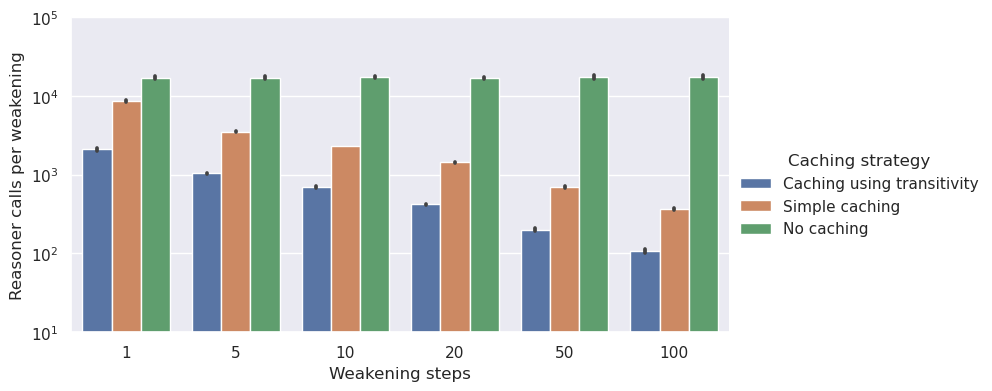
\includegraphics[width=\textwidth]{resources/calls-cache-bar.png}
  \caption{The mean number of reasoner calls needed for a single application of the axiom weakening operator, averaged over the tested ontologies.}
  \label{fig:results-cache-calls}
\end{figure}

\begin{figure}[ht]
  \centering
  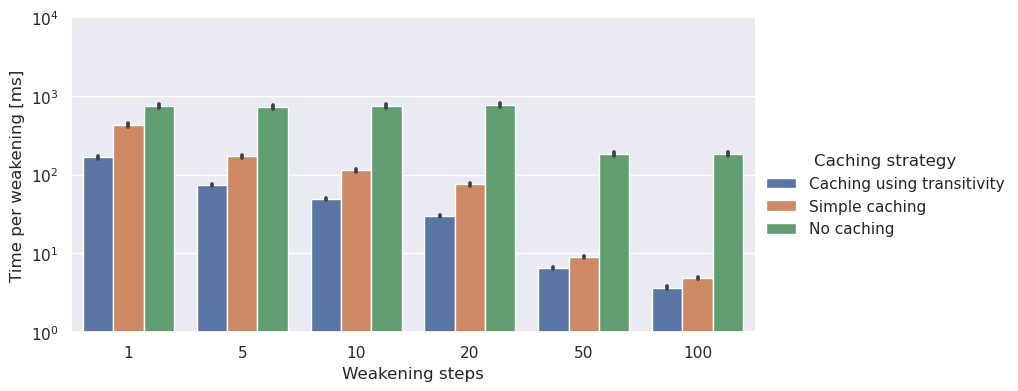
\includegraphics[width=\textwidth]{resources/time-cache-bar.png}
  \caption{Average time required per application of the axiom weakening operator with different caching strategies. The results are averaged over the tested ontologies and the reasoners FaCT++, JFact, Openllet, and HermiT.}
  \label{fig:results-cache-time}
\end{figure}

We can see clearly from the results that the cache is indeed effective at lowering both the number of reasoner calls and execution time. The simple caching method alone provides a dramatic decrease in the number of reasoner calls, especially at higher group sizes. The algorithm that can additionally exploit the transitivity of the relation performs even better, also with a smaller number of weakening steps. The difference when looking at the execution time is significantly smaller. This can likely be attributed largely to internal caching performed by the reasoners. This would also explain the observed variation when it comes to the relative improvement between different reasoners. It can be concluded that the addition of the cache greatly benefits the computation of the axiom weakening operator, especially if it can be reused for many applications of the same weakening operator.



\section{Evaluating Required Execution Time}


The performance of the axiom weakening based repair algorithm shown in \cref{algo:repair-weaken} has also been evaluated. During each repair via axiom weakening, the time taken and the number of calls to the reasoner have been registered. Additionally, the number of steps taken by the repair using axiom weakening has been observed. Also, as mentioned in \cref{eval-quality}, the repair program was put under a timeout to prevent cases where the reasoning becomes unreasonably slow. The generation of inconsistent ontologies used a similar timeout, and the same procedure was used for situations in which the reasoner ran out of memory. Timeout of the weakening procedure are shown separately from those latter cases in the results. The frequency of these cases is indicated as percentage of the overall runs finished vs started. The results of this evaluation are presented in \cref{table:results-perf} and \cref{fig:results-perf-time}.

\begin{table}[ht]
  \scriptsize
  \centering
  \begin{tabular}{|l|r@{ }lr@{ }lr@{ }lr@{ }r|}
    \cline{2-9}
    \multicolumn{1}{l|}{} & \multicolumn{2}{c}{Steps} & \multicolumn{2}{c}{Calls} & \multicolumn{2}{c}{Time [ms]} & \multicolumn{2}{c|}{Failed} \\
    \hline
    admin & 6.3 & [4.0, 9.2] & 7621 & [5601, 10118] & 9638 & [5433, 14909] & 2\% & (2\%) \\
    ahso & 2.1 & [1.7, 2.5] & 4648 & [4228, 5131] & 11469 & [8122, 15336] & 11\% & (26\%) \\
    cdao & 2.1 & [1.8, 2.5] & 16137 & [14576, 17740] & 20767 & [15204, 27269] & 19\% & (48\%) \\
    cdpeo & 1.5 & [1.3, 1.7] & 4476 & [4250, 4716] & 2050 & [1942, 2169] & 0\% & (0\%) \\
    covid19-ibo & 1.3 & [1.2, 1.5] & 14822 & [14321, 15320] & 2208 & [2126, 2296] & 4\% & (13\%) \\
    ecp & 1.3 & [1.2, 1.5] & 2020 & [1916, 2133] & 4453 & [2738, 6939] & 1\% & (14\%) \\
    emo & 1.4 & [1.3, 1.6] & 18549 & [17473, 19615] & 6582 & [4439, 9688] & 1\% & (4\%) \\
    evi & 5.0 & [3.9, 6.4] & 5955 & [4680, 7425] & 4719 & [3408, 6349] & 19\% & (64\%) \\
    falls & 1.5 & [1.3, 1.6] & 1242 & [1161, 1331] & 874 & [843, 909] & 1\% & (5\%) \\
    fo & 1.6 & [1.4, 1.8] & 1295 & [1179, 1423] & 1090 & [1025, 1164] & 38\% & (61\%) \\
    gbm & 1.5 & [1.3, 1.6] & 7608 & [7070, 8131] & 2954 & [2808, 3117] & 0\% & (0\%) \\
    gfvo & 1.8 & [1.6, 2.0] & 4167 & [3864, 4501] & 2404 & [2258, 2569] & 0\% & (0\%) \\
    koro & 1.9 & [1.7, 2.2] & 6195 & [5697, 6706] & 2456 & [2277, 2648] & 0\% & (0\%) \\
    lico & 2.6 & [2.2, 2.9] & 6638 & [6105, 7186] & 3709 & [3400, 4077] & 1\% & (22\%) \\
    mamo & 2.5 & [2.2, 2.9] & 4667 & [4228, 5128] & 2215 & [2046, 2403] & 0\% & (0\%) \\
    mpio & 2.2 & [1.8, 2.6] & 1908 & [1720, 2133] & 987 & [913, 1078] & 9\% & (30\%) \\
    pizza & 2.0 & [1.7, 2.3] & 7550 & [6723, 8419] & 26767 & [20554, 34014] & 28\% & (55\%) \\
    provo & 4.9 & [3.7, 6.3] & 6851 & [5383, 8465] & 8878 & [5962, 12348] & 4\% & (8\%) \\
    qudt & 1.1 & [1.0, 1.2] & 7044 & [6816, 7291] & 6658 & [4229, 9672] & 9\% & (38\%) \\
    trans & 3.2 & [1.8, 5.1] & 4384 & [3213, 5894] & 3684 & [1610, 6513] & 0\% & (5\%) \\
    triage & 3.2 & [2.4, 4.3] & 5166 & [4255, 6351] & 8979 & [6084, 13102] & 28\% & (51\%) \\
    vio & 2.5 & [2.1, 3.0] & 9476 & [8628, 10327] & 15199 & [10496, 20803] & 3\% & (7\%) \\
    \hline
  \end{tabular}
  \caption{Results of the evaluation with respect to performance. Number of weakening iterations, reasoner calls, and total repair time are given as sample mean, with 95\% confidence interval in brackets. The frequency of failed runs is shown as percentage of repairs by weakening that were started but not completed. In parentheses, the percentage of total failed runs, including those with timeout during generation of the inconsistent ontology. Attempts that failed were not considered for the other values.}
  \label{table:results-perf}
\end{table}

\begin{figure}[ht]
  \centering
  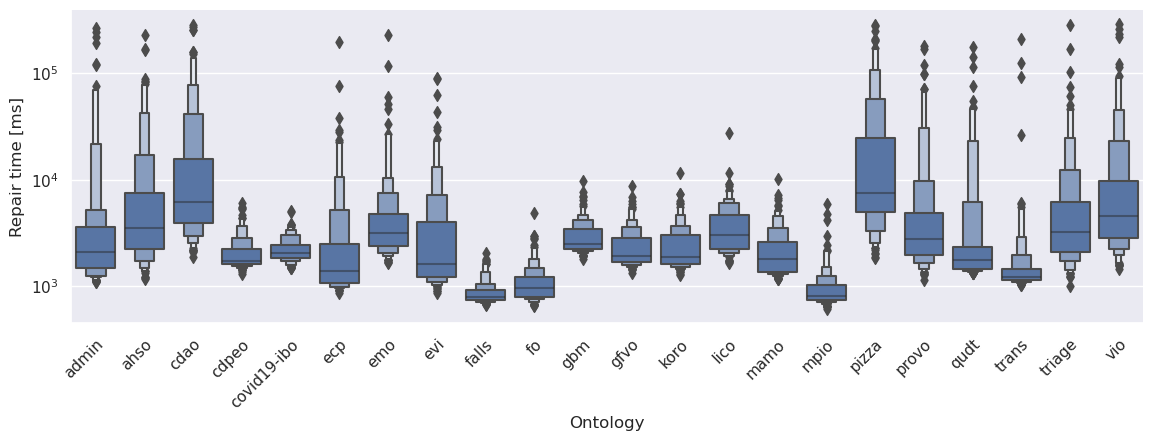
\includegraphics[width=\textwidth]{resources/time-ontology-violin.png}
  \caption{Distribution of (real) execution time required for repairing a single ontology using axiom weakening. The two darkest blue boxes represent (together) half of the samples, with the line in the middle indicating the median. Each lighter box represents half the samples of the boxes one step darker, and all remaining outliers are marked. Attempts that failed by timeout or other errors were not considered.}
  \label{fig:results-perf-time}
\end{figure}

As is visible from the results, the number of reasoner calls and the execution time can vary significantly. The execution times were generally reasonable when a run was able to complete within the time limit, with most of them completing within 2 minutes, even though the time limit was set to 5 minutes. A significant number of runs, however, were affected by the timeout or other errors. It has not been looked deeper into what causes these issues.


